\chapter{Stand der Wissenschaft}
\label{chap:forschungsstand}
Seit den Anfängen der Entwicklung von \gls{open-ran} im Februar 2016 und der Gründung der \orana{} 2018 gibt es einige wissenschaftliche Arbeiten, die sich mit dem Thema Schwachstellenanalyse und Schwachstellenbewertung in einer \gls{open-ran} Umgebung beschäftigen \autocite{ORANAlliance,GuideOpenRAN}. Unter dem Stichwort \glqq{}O-RAN\grqq{} finden sich über die \gls{mitre} \gls{cve} Suche aktuell 12 Einträge, die Schwachstellen in der O-RAN-\gls{sc}-Referenzimplementierung betreffen \autocite{CVESearchResults}. Die systematische Suche nach und Analyse von Schwachstellen ist entscheidend, um Sicherheitslücken frühzeitig zu erkennen und geeignete Gegenmaßnahmen zu implementieren. In diesem Kapitel wird ein Überblick über den Forschungsstand anhand einer Auswahl von Arbeiten gegeben.

%
\section{Technischer Report der O-RAN Alliance Security Work Group}
\label{sec:forschungsstand-wg11}
Die \gls{wg11} der \orana{} beschäftigt sich mit den sicherheitstechnischen Aspekten von \gls{open-ran} und veröffentlicht in regelmäßigen Abständen einen technischen Report, der eine Bedrohungsmodellierung und Risikobeurteilung enthält. Zum Zeitpunkt der Veröffentlichung ist der Report in Version \textit{\textsf{v04.00}} die neueste Fassung dieses Dokuments. Der Report umfasst sowohl mögliche O-RAN-spezifische Angriffe auf Komponenten und Schnittstellen in einem \gls{open-ran}-System, als auch nicht O-RAN-spezifische Bedrohungen, wie Supply-Chain-Angriffe auf quell-offenen Programmcode oder physischen Eingriff um Zugriff auf sensible Daten zu erlangen, die in allen \glspl{open-ran} existieren können \autocite{o-ranworkgroup11securityworkgroupORANSecurityThreat2024}. Im Folgenden wird ein Überblick über die O-RAN-spezifischen Bedrohungen gegeben. Die davon betroffenen Komponenten und Schnittstellen sind in Abbildung \ref{fig:oran-architecture} dargestellt.
\begin{figure}
    \centering
    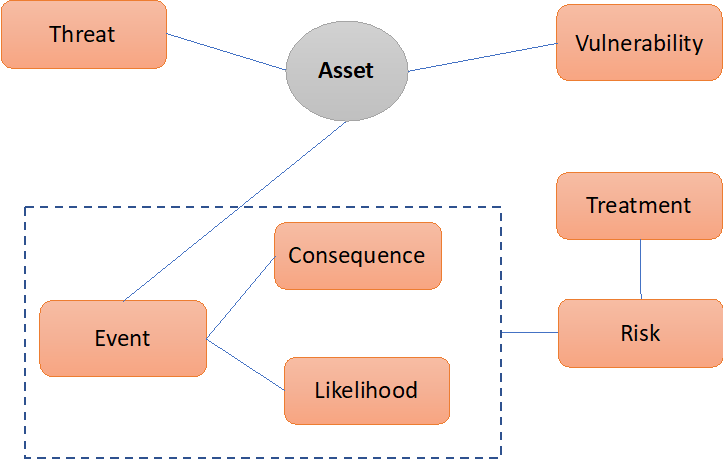
\includegraphics[width=0.5\textwidth]{oran-risk-factors}
    \caption{Einflussfaktoren für die Risikobeurteilung (Quelle: \autocite{o-ranworkgroup11securityworkgroupORANSecurityThreat2024})}
    \label{fig:oran-risk-factors}
\end{figure}
\par Es wird betrachtet wie hoch die Wahrscheinlich (\textit{Likelihood}) ist, dass eine Schwachstelle (\textit{Vulnerability}) durch eine spezifische Bedrohung (\textit{Threat}) ausgenutzt wird, und welche Konsequenzen (\textit{Consequences}) dies für das Asset hat. Die \orana{} definiert als Basis für die Risikobewertung eine Reihe von Einflussfaktoren, die in Abbildung \ref{fig:oran-risk-factors} dargestellt sind. Ein Asset ist dabei eine (Teil-)Komponente oder eine Schnittstelle zwischen Komponenten. Die \gls{wg11} identifiziert dazu 35 Bedrohungen in der Komponente \textit{O-RAN Cloud} und 69 Bedrohungen die auf alle anderen Komponenten und Schnittstellen zutreffen \autocite{o-ranworkgroup11securityworkgroupORANSecurityThreat2024}. Die \orana{} definiert in ihrem Bericht 102 kritische Assets, also solche, die besonders vor Beeinflussung in den Bereichen Integrität, Verfügbarkeit, Vertraulichkeit, Wiederholbarkeit und Authentizität geschützt werden müssen. Die Verbindung zwischen Bedrohungen und kritischen Assets wird im Bedrohungsinventar hergestellt. Aus der Schweregradbeurteilung und der Eintrittwahrscheinlichkeitsbeurteilung wird der finale Risikowert berechnet. Die Verbindung zwischen einer spezifischen Bedrohung und dem zugehörigen Risikowert stellt das Ergebnis der Risikobewertung dar.
\par Dieser Report gibt keine subjektive Bewertung darüber ab, wie risikobehaftet die Komponenten im System sind. Es handelt sich um eine rein objektive Bewertung, die durch einen Risikowert festgelegt ist. Der Risikowert setzt sich zusammen aus dem Schweregrad und der Wahrscheinlich der Ausnutzung. Der Großteil der Bedrohungen wird dabei in der Risikobewertung mit einem Risikowert von \textit{High} eingestuft, vergleiche Abbildung \ref{fig:riskscore-oran-components} \autocite{o-ranworkgroup11securityworkgroupORANSecurityThreat2024}.
%
\begin{figure}
    \centering
    \label{fig:riskscore-oran-components}
    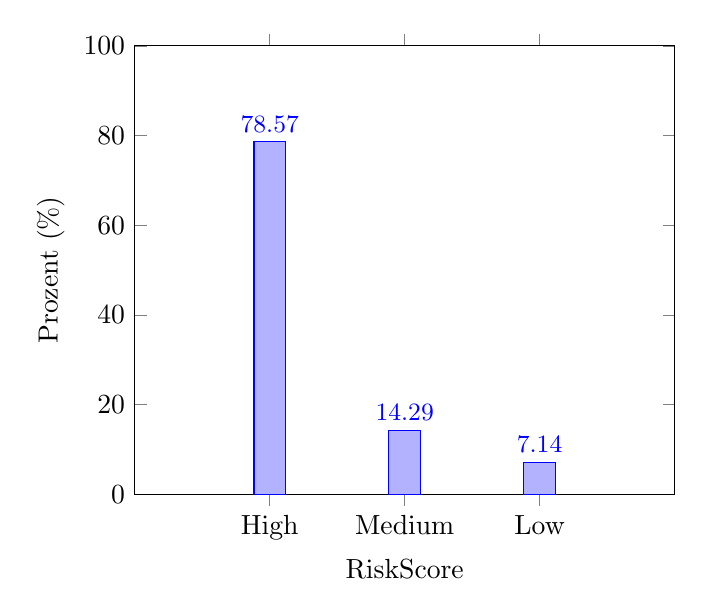
\begin{tikzpicture}
        \begin{axis}[
                ybar,
                symbolic x coords={High, Medium, Low},
                xtick=data,
                ymin=0, ymax=100,
                ylabel={Prozent (\%)},
                xlabel={RiskScore},
                nodes near coords,
                every node near coord/.append style={font=\small},
                bar width=0.4cm,
                enlarge x limits=0.5
            ]
            \addplot coordinates {(High, 78.57) (Medium, 14.29) (Low, 7.14)};
        \end{axis}
    \end{tikzpicture}
    \caption{Risikobewertung der Bedrohungen in O-RAN Komponenten und Schnittstellen}
\end{figure}
%

\section{BSI Risikoanalyse}
\label{sec:forschungsstand-bsi}
In der Studie des Bundesamts für Sicherheit in der Informationstechnik (BSI) wird eine weitere Risikoanalyse durchgeführt. Die Studie zielt dabei nicht darauf ab, spezifische Schwachstellen in der Implementierung, sondern in den Spezifikationen der \orana{} zu finden. \citeauthor{kopsellOpenRANRisikoanalyse2022} führen an, dass die veröffentlichten O-RAN-Spezifikationen zum Zeitpunkt Februar 2022 nicht viele Vorgaben zur Sicherheit machen und sich insbesondere nicht an dem Ansatz \textit{security/privacy by design/default} orientiert. Als Folge dessen werden viele potenzielle Sicherheitsrisiken mit mittlerem bis hohem Schweregrad festgestellt. Die Studie präsentiert Maßnahmen, deren Umsetzung zur Verbesserung der Sicherheit in der O-RAN-Umgebung führen würde. \citeauthor{kopsellOpenRANRisikoanalyse2022} betonen dabei die Dringlichkeit, diese Maßnahmen in einem möglichst frühen Stadium in den Spezifikationen zu berücksichtigen \autocite{kopsellOpenRANRisikoanalyse2022}.
\par Weitere umfangreiche Risikoanalysen für 5G oder 5G RAN wurden von Network
and Information Systems Cooperation Group (NIS) und The European Union
Agency for Cybersecurity (ENISA) veröffentlicht, diese sind aber nicht auf Open
RAN fokussiert [13,14].
%
\section{Empirische Analyse von Schwachstellen im Open RAN Umfeld}
\label{sec:forschungsstand-acema}
\citeauthor{klementSecuring6GTransition2024} untersuchen in ihrem Artikel \textit{Toward Securing the 6G Transition: A Comprehensive Empirical Method to Analyze Threats in O-RAN Environments} (ACEMA) die Sicherheitsherausforderungen, die mit dem Übergang von 5G zu 6G-Netzen und der Einführung von \gls{open-ran}-Technologien einhergehen. Ziel ihrer Forschung ist die Entwicklung eines umfassenden Ansatzes zur Analyse von Sicherheitsbedrohungen in \gls{open-ran} Umgebungen. Hierzu kombinieren die Autoren das \gls{mitre} \gls{attack} Framework mit empirischen Daten, um Bedrohungen in einer O-RAN-Implementierung zu analysieren. Im Zentrum ihrer Methodik steht die Abbildung einer \gls{mitre}-Technik zu einem spezifischen \gls{cve}-Datum über das Durchsuchen der unterschiedlichen Kategorisierungssysteme \gls{capec}, \gls{cwe} und \gls{cve}. Die Anwendung des \gls{cvss}, um den Schweregrad möglicher Schwachstellen zu bewerten, geht über die bisher vorgenommenen Bewertungssysteme der \orana{} heraus und ermöglicht eine granuläre Auswertung der Ergebnisse. Die Erkenntnisse von \citeauthor{klementSecuring6GTransition2024} tragen dazu bei, ein erhöhtes Bewusstsein für spezifische Bedrohungsszenarien und vulnerable O-RAN Komponenten zu schaffen. Dies wird durch einfach verständliche Datenvisualisierungen erreicht \autocite{klementSecuring6GTransition2024}.

%
\section{Empirische Analyse von Schwachstellen im Android Umfeld}
\label{sec:forschungsstand-android}
Auch in anderen Feldern der Informatik werden empirische Methoden genutzt, um die Sicherheit von Komponenten im jeweiligen System zu analysieren und bewerten.
\par Mit \citetitle{mazuera-rozoAndroidOSStack2019} wurde 2019 eine empirische Studie durchgeführt die, ähnlich wie \gls{acema} im Umfeld von \gls{open-ran}, eine umfangreiche Schwachstellenanalyse und Schwachstellenbewertung auf allen öffentlich auffindbaren Schwachstellen im Android-Umfeld betrachtet. \citeauthor{mazuera-rozoAndroidOSStack2019} betrachten in dieser Studie besonders die Art der Schwachstellen und wie sich diese über den Verlauf der Zeit ändert. Außerdem werden die Angriffsvektoren nach \gls{cvss} analysiert, die angegriffenen Ebenen und Teilsysteme von Android betrachtet und die Frage beantwortet, wie lange es dauert, bis die Schwachstellen geschlossen werden. Die Studie nutzt die \gls{mitre} \gls{cwe} Kategorisierung, um die spezifischen Schwachstellen einer übergeordneten Schwachstellenkategorie zuzuordnen. Sie kommen zu dem Schluss, dass mindestens 60\% der 1235 betrachteten Schwachstellen eine hohe Auswirkung auf die Vertraulichkeit(60\%), Integrität(60\%) und Verfügbarkeit(65\%) des Geräts haben \autocite{mazuera-rozoAndroidOSStack2019}. Diese Studie zeigt, wie auch die Studie von \citeauthor{klementSecuring6GTransition2024}, den wissenschaftlichen Nutzen einer empirischen Analyse.